\documentclass[border=4pt]{standalone}
\usepackage{amsmath,amssymb}
\usepackage{pgfplots}
\pgfplotsset{compat=1.17,
  colormap={gr}{rgb255=(240,240,240) rgb255=(160,160,160)},
  colormap={bl}{rgb255=(205,222,248) rgb255=(60,100,185)},
  colormap={o}{rgb255=(250,226,200) rgb255=(205,120,60)}}
\usetikzlibrary{arrows.meta,calc}
\begin{document}
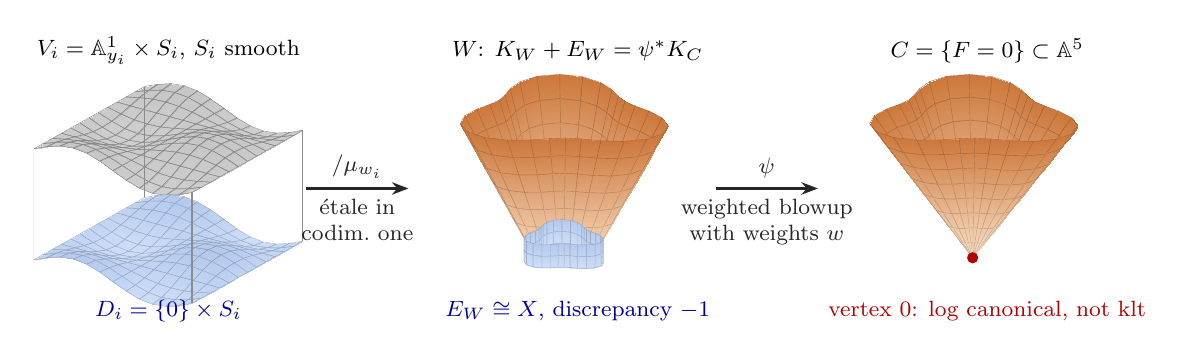
\begin{tikzpicture}[
  arrowstep/.style={-{Stealth[length=6pt]},line width=0.8pt,gray!30!black},
  lab/.style={font=\footnotesize,align=center}]
% ---------- (a) the chart V_i = A^1 x S_i with D_i = {0} x S_i ----------
\begin{axis}[at={(0cm,0cm)},anchor=center,width=5.0cm,height=5.0cm,hide axis,
  view={35}{25},z buffer=sort,zmin=-0.3,zmax=2.2]
  \addplot3[surf,shader=faceted interp,colormap name=gr,draw=black!25,line width=0.15pt,fill opacity=0.6,samples=13,domain=-1:1,y domain=-1:1]
    (x,y,{1.7+0.18*sin(180*x)*cos(180*y)});
  \addplot3[surf,shader=faceted interp,colormap name=bl,draw=blue!50!black,line width=0.15pt,samples=13,domain=-1:1,y domain=-1:1]
    (x,y,{0.18*sin(180*x)*cos(180*y)});
  \foreach \a/\b in {-1/-1,1/-1,1/1,-1/1}{
    \edef\temp{\noexpand\addplot3[black!45,line width=0.5pt,domain=0:1.7,samples=2] (\a,\b,x);}
    \temp}
\end{axis}
\node[lab,blue!60!black] at (0,-1.55) {$D_i=\{0\}\times S_i$};
\node[lab] at (0,1.75) {$V_i=\mathbb A^1_{y_i}\times S_i$, $S_i$ smooth};
\draw[arrowstep] (1.75,0)--node[lab,above]{$/\mu_{w_i}$}node[lab,below]{\'etale in\\ codim.\ one}(3.05,0);
% ---------- (b) the weighted blowup W with E_W ----------
\begin{axis}[at={(5.2cm,0cm)},anchor=center,width=5.0cm,height=5.0cm,hide axis,
  view={30}{22},z buffer=sort]
  \addplot3[surf,shader=faceted interp,colormap name=o,draw=black!30,line width=0.15pt,samples=31,samples y=7,domain=0:360,y domain=0.38:1]
    ({y*cos(x)*(1+0.22*cos(3*x))},{y*sin(x)*(1+0.22*cos(3*x))},{y});
  \addplot3[surf,shader=faceted interp,colormap name=bl,draw=blue!50!black,line width=0.15pt,samples=31,samples y=3,domain=0:360,y domain=0.26:0.38]
    ({0.38*cos(x)*(1+0.22*cos(3*x))},{0.38*sin(x)*(1+0.22*cos(3*x))},{y});
\end{axis}
\node[lab,blue!60!black] at (5.2,-1.55) {$E_W\cong X$, discrepancy $-1$};
\node[lab] at (5.2,1.75) {$W$: $K_W+E_W=\psi^*K_C$};
\draw[arrowstep] (6.95,0)--node[lab,above]{$\psi$}node[lab,below]{weighted blowup\\ with weights $w$}(8.25,0);
% ---------- (c) the cone C ----------
\begin{axis}[at={(10.4cm,0cm)},anchor=center,width=5.0cm,height=5.0cm,hide axis,
  view={30}{22},z buffer=sort]
  \addplot3[surf,shader=faceted interp,colormap name=o,draw=black!30,line width=0.15pt,samples=31,samples y=9,domain=0:360,y domain=0:1]
    ({y*cos(x)*(1+0.22*cos(3*x))},{y*sin(x)*(1+0.22*cos(3*x))},{y});
  \addplot3[only marks,mark=*,mark size=1.8pt,red!70!black] coordinates {(0,0,0)};
\end{axis}
\node[lab,red!70!black] at (10.4,-1.55) {vertex $0$: log canonical, not klt};
\node[lab] at (10.4,1.75) {$C=\{F=0\}\subset\mathbb A^5$};
\end{tikzpicture}
\end{document}
